\begin{myposter}{
    Глава 2. Результаты расчетов. Движения 1 и 2.
}

    \headerbox
    {Движение 1 ($\nu_{1,2}(0) = 0, \nu_3 = 1$)}
    {name=first,column=0,row=0,span=3}
    {
        {\huge\bf
            \vspace{10pt}
            \begin{figure}[H]
                \centering
                \minipage{0.33\textwidth}
                    \centering
                    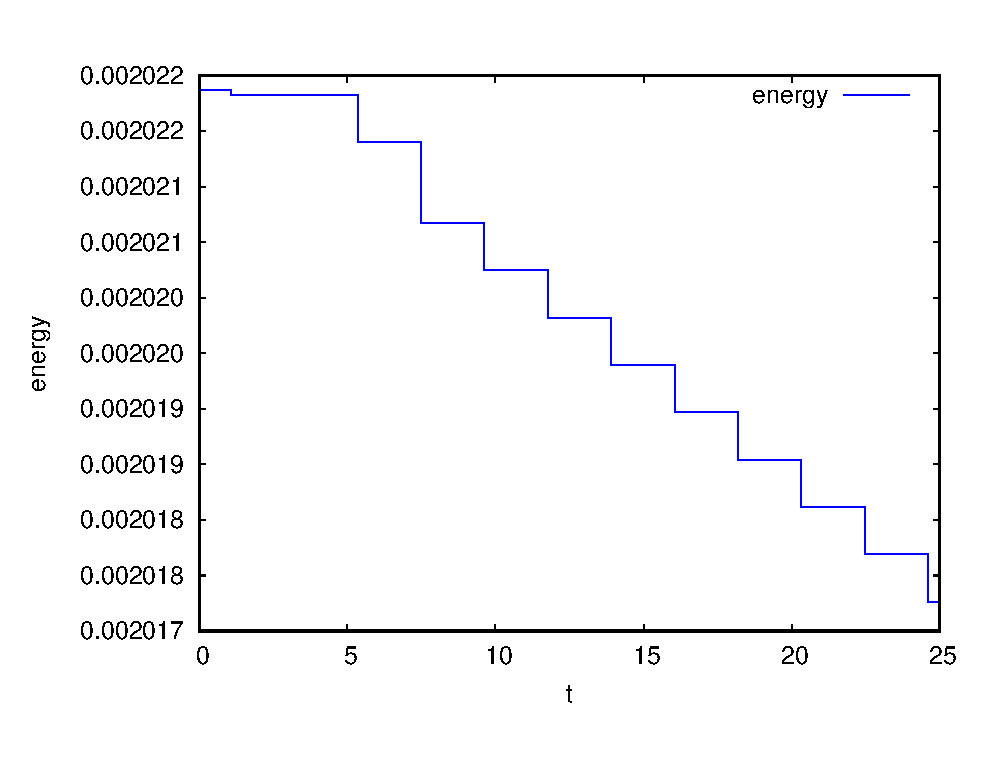
\includegraphics[width=\linewidth]{content/pic/self_rot_25/kin_en.eps}
                    \vspace{-15pt}
                    \caption{Кинетическая энергия}
                \endminipage
                \minipage{0.33\textwidth}
                    \centering
                    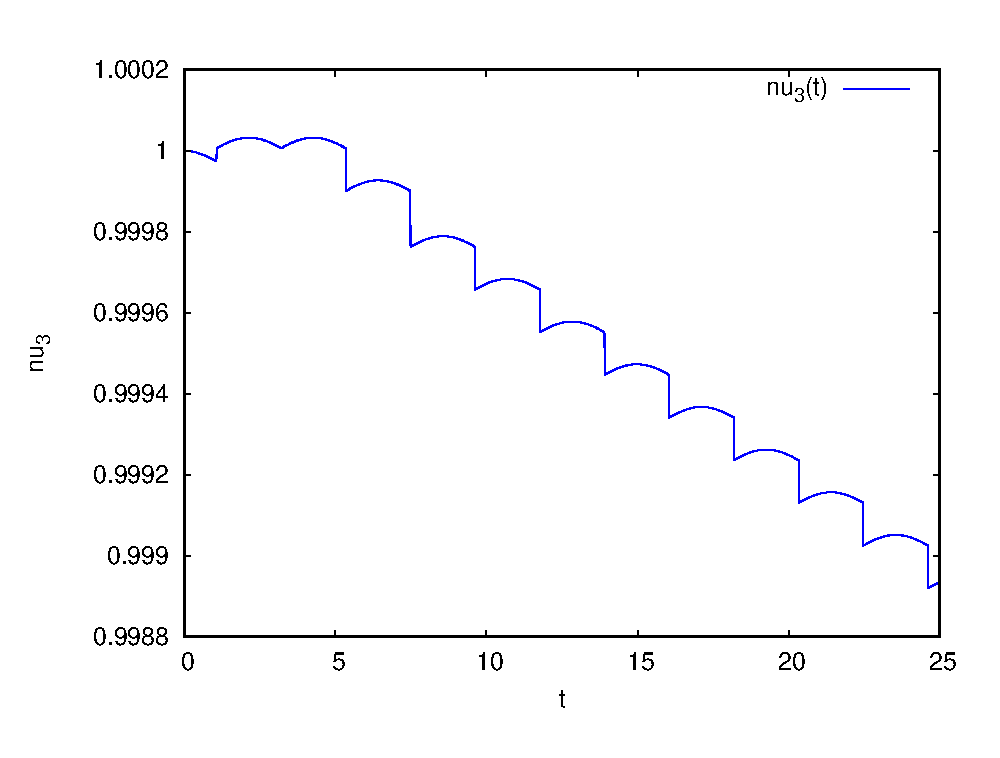
\includegraphics[width=\linewidth]{content/pic/self_rot_25/nu3.eps}
                    \vspace{-15pt}
                    \caption{Угловая скорость экипажа}
                \endminipage
                \minipage{0.33\textwidth}
                    \centering
                    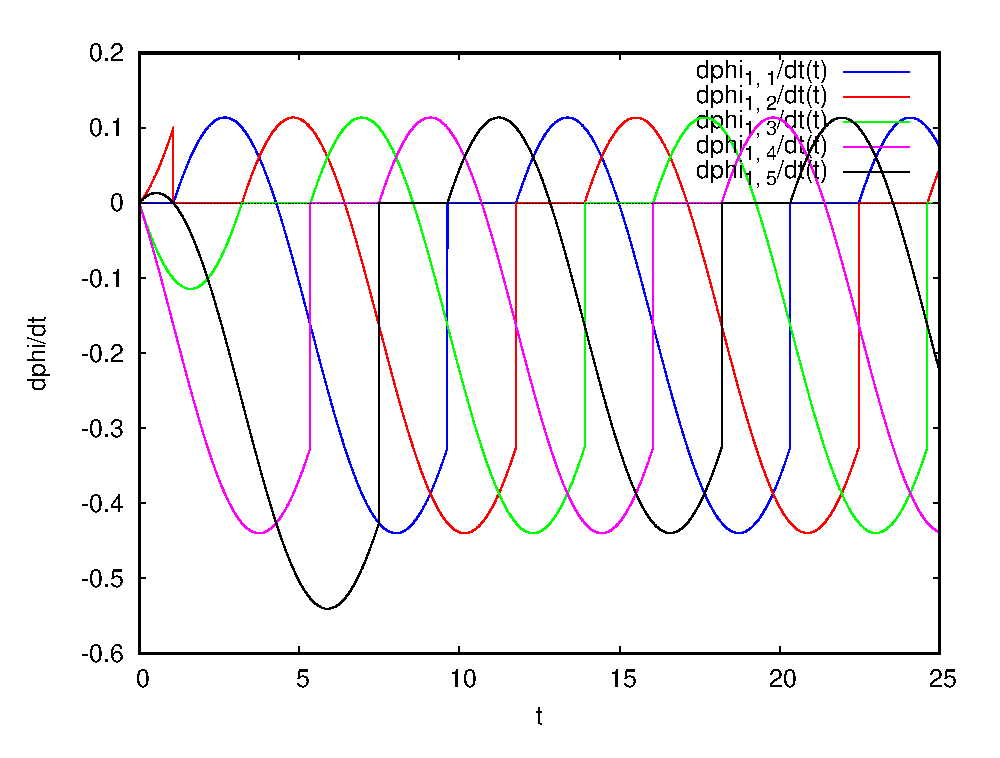
\includegraphics[width=\linewidth]{content/pic/self_rot_25/rol_vel.eps}
                    \vspace{-15pt}
                    \caption{Угловые скорости роликов}
                \endminipage
            \end{figure}
            \vspace{10pt}
        }
    }
    
    \headerbox
    {Движение 2 ($\nu_1(0) = 1, \nu_{2,3} = 0$)}
    {name=second,column=0,row=1,below=first,span=3}
    {
        {\huge\bf
            \vspace{10pt}
            \centering
            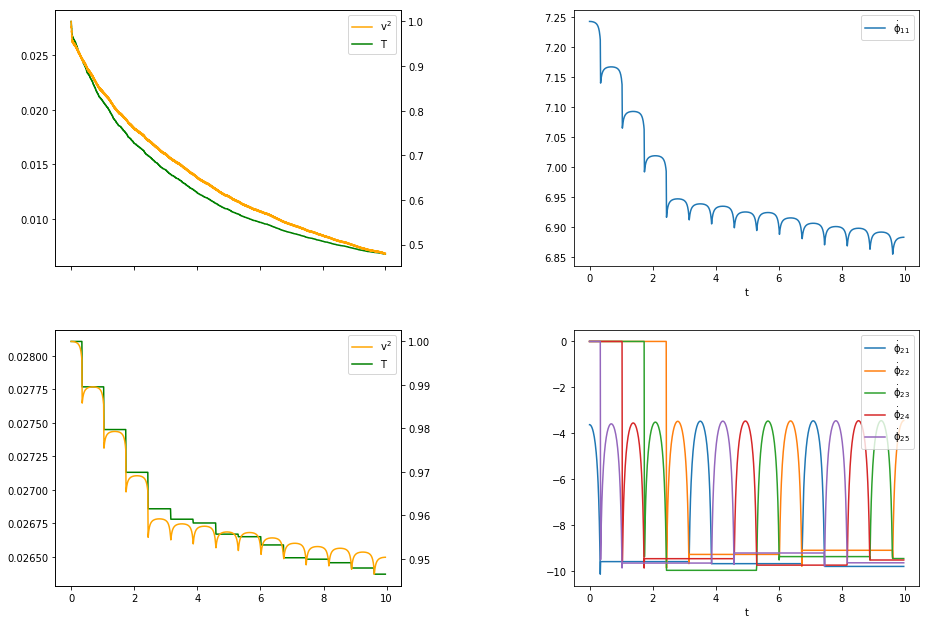
\includegraphics[width=\linewidth]{content/pic/new/impact_2.png}
            \vspace{10pt}
        }
    }
    
\end{myposter}
